%\begin{frame}
%    \frametitle{Научная новизна}
%    \begin{itemize}
%        \item Впервые реализован \dots
%        \item Разработана программа \dots
%        \item Впервые проведён анализ \dots
%        \item Предложена схема \dots
%    \end{itemize}
%\end{frame}
%\note{
%    Проговаривается вслух научная новизна
%}
%
%\begin{frame}
%    \frametitle{Научная и практическая значимость}
%    \begin{itemize}
%        \item Получены выражения для \dots.
%        \item Определены условия \dots.
%        \item Разработаны устройства \dots.
%    \end{itemize}
%\end{frame}
%\note{
%    Проговариваются вслух научная и практическая значимость
%}
%
%\begin{frame}
%    \frametitle{Свидетельство о регистрации программы}
%    \begin{figure}[h]
%        \centering
%        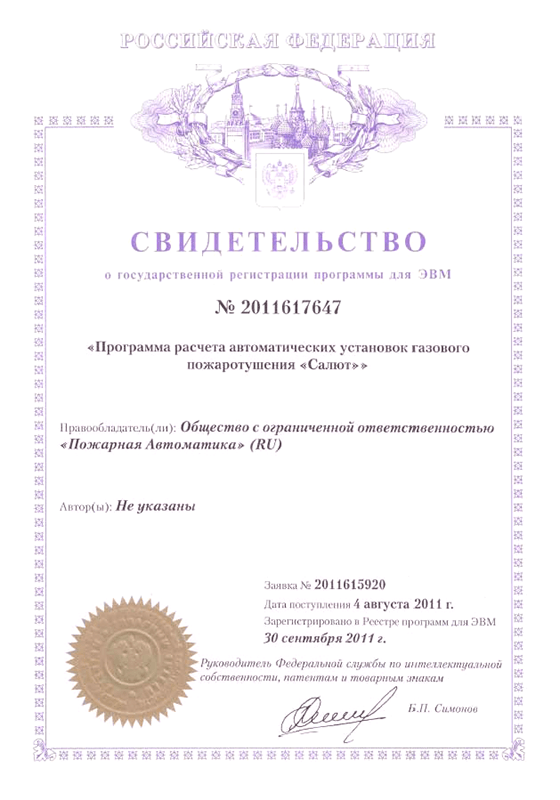
\includegraphics[height=0.7\textheight]{registration}
%    \end{figure}
%\end{frame}
%\note{
%    Получено свидетельство о регистрации разработанной программы \textsc{Hello~world™}.
%}
%
%\begin{frame}
%    \frametitle{Акт о внедрении}
%    \begin{figure}[h]
%        \centering
%        \fbox{
%            \begin{minipage}[t]{0.4\linewidth}
%                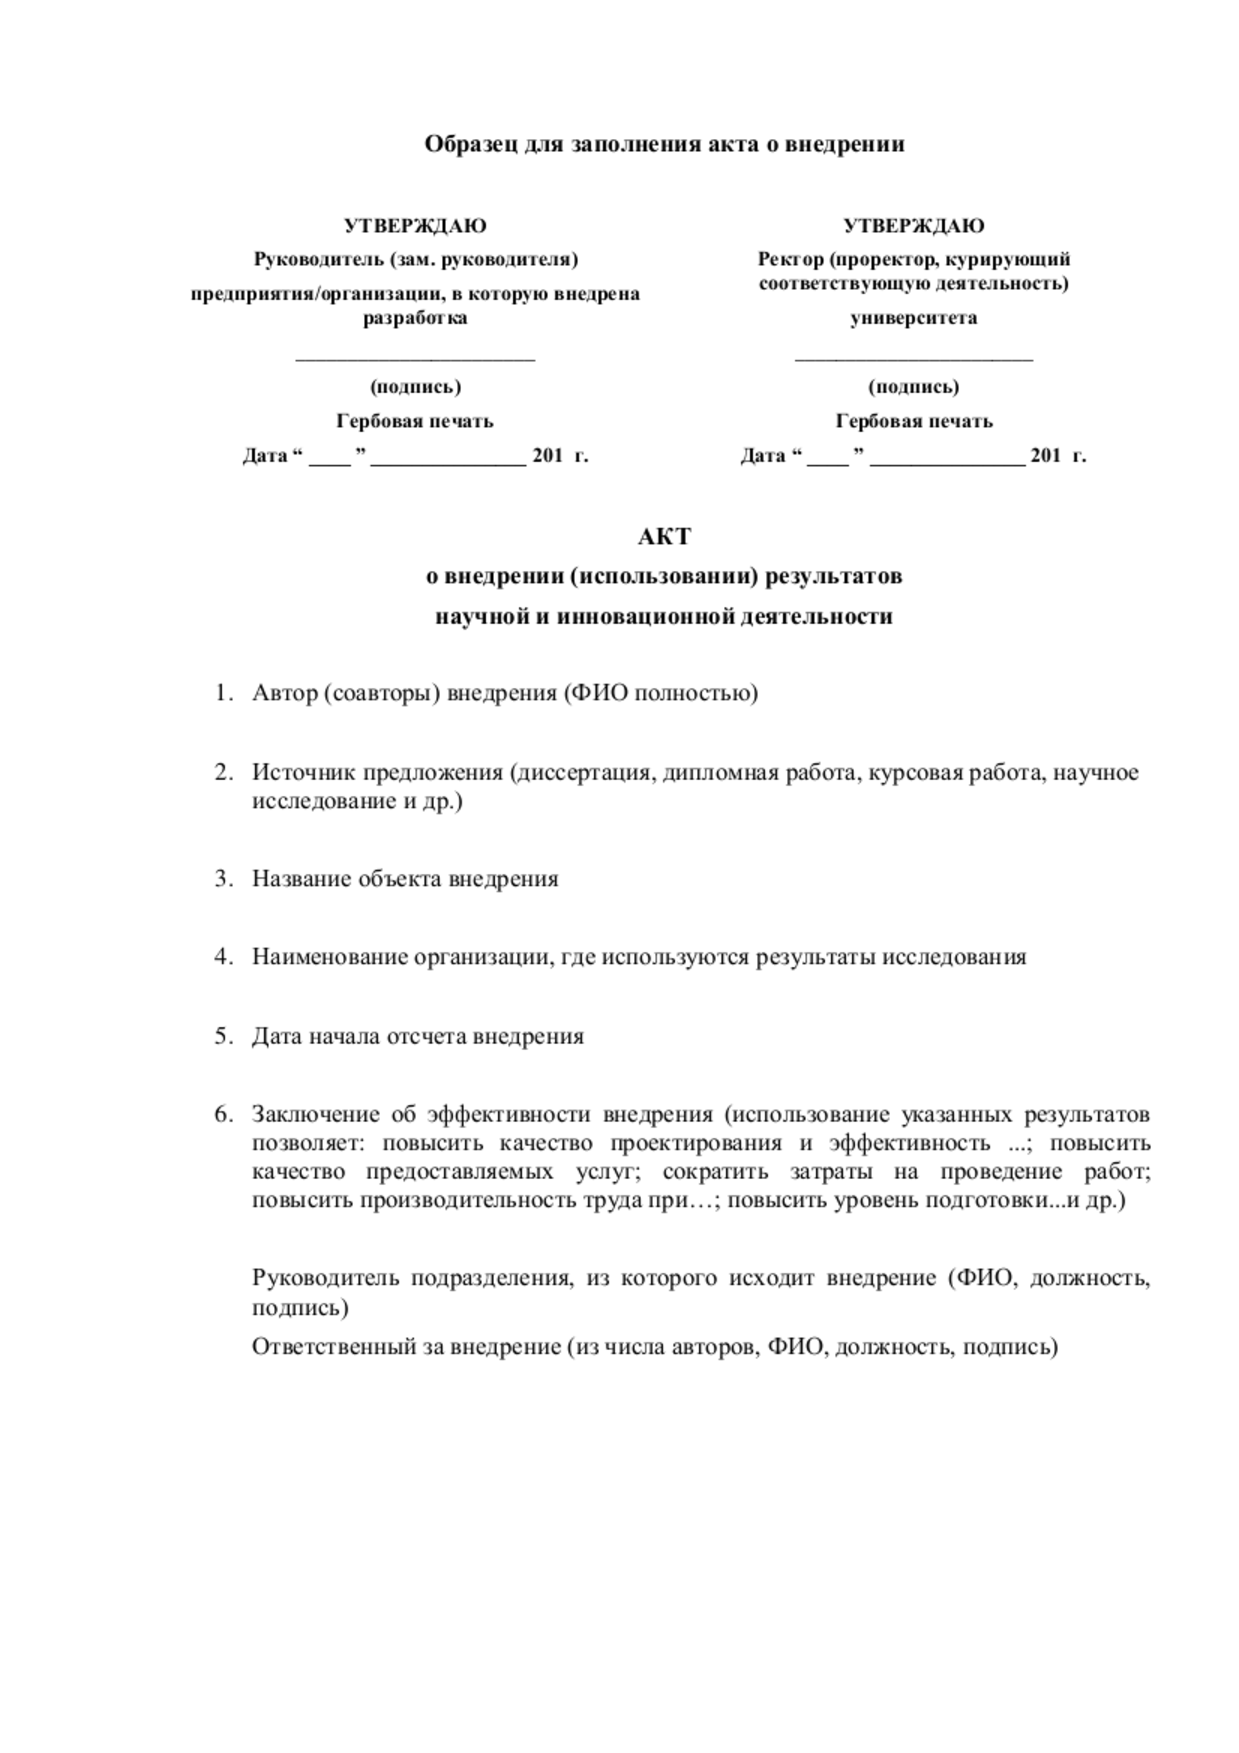
\includegraphics[width=\linewidth]{implementation}
%            \end{minipage}
%        }
%    \end{figure}
%\end{frame}
%\note{
%    Получен акт о внедрении.
%}

% \begin{frame} % публикации на одной странице
%\begin{frame}[t,allowframebreaks] % публикации на нескольких страницах
%    \frametitle{Основные публикации}
%    \nocite{vakbib1}%
%    \nocite{vakbib2}%
%    %
%    %% authorwos
%    \nocite{wosbib1}%
%    %
%    %% authorscopus
%    \nocite{scbib1}%
%    %
%    %% authorconf
%    \nocite{confbib1}%
%    \nocite{confbib2}%
%    %
%    %% authorother
%    \nocite{bib1}%
%    \nocite{bib2}%
%    \ifnumequal{\value{bibliosel}}{0}{
%        \insertbiblioauthor
%    }{
%        \printbibliography%
%    }
%\end{frame}
%\note{
%    Результаты работы опубликованы в N печатных изданиях, в т.ч. M реферируемых изданиях.
%}

\begin{frame}
    \frametitle{Участие в конференциях}
    \begin{itemize}
    	\item IV Всероссийская научно-техническая конференция аспирантов, магистрантов и молодых ученых с международным участием «Молодые ученые -- ускорению научно-технического прогресса в XXI веке». (Ижевск, 2016).
    	\item Шестая международная конференция «Geometry, Dynamics, Integrable Systems -- GDIS 2016» (Ижевск, 2016 г.)
    	\item Машиноведение и инновации. Конференция молодых учёных и студентов (МИКМУС-2018) (Москва, 2018 г.)
    	\item International Conference "Scientific Heritage of Sergey A. Chaplygin: nonholonomic mechanics, vortex structures and hydrodynamics" (Чебоксары, 2019 г.)
    	\item 30-я международная научно-техническая конференция "Экстремальная робототехника-2019" (Санкт-Петербург, 2019 г.)	
    \end{itemize}
\end{frame}

\begin{frame}
\frametitle{Публикации}
\begin{itemize}
	
	\item Ветчанин Е. В, Караваев Ю.Л., Калинкин А.А., Пивоварова Е.Н., Клековкин А.В. Модель безвинтового подводного робота //Вестник Удмуртского университета. Математика. Механика. Компьютерные науки. – 2015. – Т. 25. – №. 4. – С. 544-553. (ВАК)
	
	\item Karavaev Y. L., Kilin A. A., Klekovkin A. V. Experimental investigations of the controlled motion of a screwless underwater robot // Regular and Chaotic Dynamics. – 2016. – Т. 21. – №. 7-8. – С. 918-926 (WoS)
	
	\item Klekovkin A.V., Karavaev Yu.L., Kilin A.A., Mamaev I.S. Control screwless fish-like robot with internal rotor // Extreme Robotics,  2019, Vol.1, no. 1, pp. 220-225 (РИНЦ)
	
	\item Yury Karavaev, Anton Klekovkin, Ivan Mamaev, Valentin Tenenev, Eugene Vetchanin, "A Simple Physical Model for Control of an Propellerless Aquatic Robot",  Mechanical Systems and Signal Processing, 2020, unpublished.
		
\end{itemize}
\end{frame}

\begin{frame}
\frametitle{Патенты}
\begin{itemize}
	
%	\item № 2015615728. Программа для управления безвинтовым надводным роботом // А.В. Борисов, И.С. Мамаев, А.А. Килин, Ю.Л. Караваев, А.В. Клековкин, А.В. Шелухо, А.И. Кленов, Е.В. Ветчанин, В.А. Тененев. Заявитель и патентообладатель – ФБГОУ ВО «ИжГТУ имени М.Т. Калашникова»; Заявка: 2015612643, 07.04.2015, опубл. 22.05.2015
	
	
	\item Патент на полезную модель. №172254 РФ. Безвинтовой подводный робот //  А.В. Борисов, И.С. Мамаев, А.А. Килин, А.А. Калинкин, Ю.Л. Караваев, А.В. Клековкин, Е.В. Ветчанин; заявитель и патентообладатель – ФБГОУ ВО «ИжГТУ имени М.Т. Калашникова»; Заявка: 2016144812, 15.11.2016, опубл. 3.07.2017
	
	
	\item № 2017613219. Программа для управления безвинтовым подводным роботом // А.В. Борисов, И.С. Мамаев, А.А. Килин, Ю.Л. Караваев, А.В. Клековкин. Заявитель и патентообладатель – ФБГОУ ВО «ИжГТУ имени М.Т. Калашникова»; Заявка: 2016662663, 22.11.2016, опубл. 16.03.2017
	
	
	\item № 2019612284. Программа управления безвинтовым надводным роботом с внутренним ротором // А.В. Борисов, И.С. Мамаев, А.А. Килин, А.В. Клековкин, Ю.Л. Караваев. Заявитель и патентообладатель – ФБГОУ ВО "ИжГТУ имени М.Т. Калашникова"; Заявка: 2019610925, 04.02.2019, опубл. 14.02.2019
	
	
\end{itemize}
\end{frame}

%\note{
%    Работа была представлена на ряде конференций.
%}
%
%\begin{frame}[plain, noframenumbering] % последний слайд без оформления
%    \begin{center}
%        \Huge
%        Спасибо за внимание!
%    \end{center}
%\end{frame}
